\documentclass{beamer}
\usepackage[utf8]{inputenc}
\usepackage{graphicx, epsfig}
\usepackage{amsmath,mathrsfs,amsfonts,amssymb}
\usepackage{floatflt}
\usepackage{epic,ecltree}
\usepackage{mathtext}
\usepackage{fancybox}
\usepackage{fancyhdr}
\usepackage{multirow}
\usepackage{enumerate}
\usepackage{epstopdf}
\usepackage{multicol}
\usepackage{algorithm}
\usepackage[noend]{algorithmic}
\usepackage{tikz}
\usepackage{blindtext}
\usetheme{default}%{Singapore}%{Warsaw}%{Warsaw}%{Darmstadt}
\usecolortheme{default}

\setbeamerfont{title}{size=\Huge}
\setbeamertemplate{footline}[page number]{}

\setbeamertemplate{section in toc}[sections numbered]


\makeatletter
\newcommand\HUGE{\@setfontsize\Huge{35}{40}}
\makeatother    

\setbeamerfont{title}{size=\HUGE}
\beamertemplatenavigationsymbolsempty

% latin bold lower
\newcommand{\ba}{\mathbf{a}} 
\newcommand{\bc}{\mathbf{c}} 
\newcommand{\be}{\mathbf{e}} 
\newcommand{\bff}{\mathbf{f}} % \bf - for bold type
\newcommand{\bg}{\mathbf{g}} 
\newcommand{\bh}{\mathbf{h}} 
\newcommand{\bp}{\mathbf{p}} 
\newcommand{\bq}{\mathbf{q}} 
\newcommand{\bt}{\mathbf{t}} 
\newcommand{\bs}{\mathbf{s}} 
\newcommand{\bu}{\mathbf{u}} 
\newcommand{\bv}{\mathbf{v}} 
\newcommand{\bw}{\mathbf{w}} 
\newcommand{\bx}{\mathbf{x}} 
\newcommand{\by}{\mathbf{y}} 
\newcommand{\bz}{\mathbf{z}} 

% latin bold upper
\newcommand{\bA}{\mathbf{A}} 
\newcommand{\bB}{\mathbf{B}} 
\newcommand{\bC}{\mathbf{C}} 
\newcommand{\bG}{\mathbf{G}} 
\newcommand{\bI}{\mathbf{I}} 
\newcommand{\bJ}{\mathbf{J}} 
\newcommand{\bL}{\mathbf{L}} 
\newcommand{\bM}{\mathbf{M}} 
\newcommand{\bP}{\mathbf{P}}
\newcommand{\bQ}{\mathbf{Q}} 
\newcommand{\bR}{\mathbf{R}} 
\newcommand{\bT}{\mathbf{T}} 
\newcommand{\bU}{\mathbf{U}} 
\newcommand{\bV}{\mathbf{V}} 
\newcommand{\bW}{\mathbf{W}} 
\newcommand{\bX}{\mathbf{X}} 
\newcommand{\bY}{\mathbf{Y}} 
\newcommand{\bZ}{\mathbf{Z}} 

% latin cal upper
\newcommand{\cF}{\mathcal{F}} 
\newcommand{\cG}{\mathcal{G}} 
\newcommand{\cI}{\mathcal{I}} 
\newcommand{\cL}{\mathcal{L}} 
\newcommand{\cM}{\mathcal{M}} 
\newcommand{\cN}{\mathcal{N}} 
\newcommand{\cP}{\mathcal{P}} 
\newcommand{\cS}{\mathcal{S}} 
\newcommand{\cT}{\mathcal{T}} 
\newcommand{\cW}{\mathcal{W}} 
\newcommand{\cX}{\mathcal{X}} 
\newcommand{\cZ}{\mathcal{Z}} 

% latin bb upper
\newcommand{\bbE}{\mathbb{E}} 
\newcommand{\bbI}{\mathbb{I}} 
\newcommand{\bbP}{\mathbb{P}} 
\newcommand{\bbR}{\mathbb{R}} 

% greek bold lower
\newcommand{\bepsilon}{\boldsymbol{\epsilon}} 
\newcommand{\btheta}{\boldsymbol{\theta}} 
\newcommand{\blambda}{\boldsymbol{\lambda}} 
\newcommand{\bpi}{\boldsymbol{\pi}} 
\newcommand{\bmu}{\boldsymbol{\mu}} 
\newcommand{\bsigma}{\boldsymbol{\sigma}} 
\newcommand{\bphi}{\boldsymbol{\phi}} 

% greek bold upper
\newcommand{\bSigma}{\boldsymbol{\Sigma}} 

\DeclareMathOperator*{\argmin}{arg\,min}
\DeclareMathOperator*{\argmax}{arg\,max}
\newcommand{\createdgmtitle}[1]{\title[\hbox to 56mm{Deep Generative Models  \hfill\insertframenumber\,/\,\inserttotalframenumber}]
	{\vspace{1cm} \\ \textbf{Deep Generative Models} \\ {\Huge Lecture #1}}
	\author{Roman Isachenko}
		\institute{
\includegraphics[width=0.7cm]{../utils/aimasterslogo} \LARGE{AI Masters}}
	\date{2025, Spring}
}

\usepackage{tikz}
\usetikzlibrary{arrows,shapes,positioning,shadows,trees}

\newcommand\myfootnote[1]{%
  \tikz[remember picture,overlay]
  \draw (current page.south west) +(1in + \oddsidemargin,0.5em)
  node[anchor=south west,inner sep=0pt]{\parbox{\textwidth}{%
      \rlap{\rule{10em}{0.4pt}}\raggedright\scriptsize \textit{#1}}};}

\newcommand\myfootnotewithlink[2]{%
  \tikz[remember picture,overlay]
  \draw (current page.south west) +(1in + \oddsidemargin,0.5em)
  node[anchor=south west,inner sep=0pt]{\parbox{\textwidth}{%
      \rlap{\rule{10em}{0.4pt}}\raggedright\scriptsize\href{#1}{\textit{#2}}}};}
      
\AtBeginSection[]
      {
      	\begin{frame}{Outline}
      		\tableofcontents[currentsection]
      	\end{frame}
      }
      \AtBeginSubsection[]{
      	\begin{frame}{Outline}
      		\tableofcontents[currentsection,currentsubsection]
      	\end{frame}
}
\createdgmtitle{13}

%--------------------------------------------------------------------------------
\begin{document}
%--------------------------------------------------------------------------------
\begin{frame}[noframenumbering,plain]
%\thispagestyle{empty}
\titlepage
\end{frame}
%=======
\begin{frame}{Recap of previous lecture}
	\vspace{-0.3cm}
	\[
		d\bx = \mathbf{f}(\bx, t) dt + g(t) d \bw
	\]
	\vspace{-0.3cm}
	\begin{block}{Variance Exploding SDE (NCSN)}
		\vspace{-0.5cm}
		\[
			d \bx = \sqrt{\frac{ d [\sigma^2(t)]}{dt}} \cdot d \bw, \quad \bff(\bx, t) = 0, \quad g(t) = \sqrt{\frac{ d [\sigma^2(t)]}{dt}} 
		\]
		Variance grows since $\sigma(t)$ is a monotonically increasing function.
	\end{block}
	\begin{block}{Variance Preserving SDE (DDPM)}
		\vspace{-0.3cm}
		\[
			d \bx = - \frac{1}{2} \beta(t) \bx(t) dt + \sqrt{\beta(t)} \cdot d \bw
		\]
		\[
			\bff(\bx, t) = - \frac{1}{2} \beta(t) \bx(t) , \quad g(t) = \sqrt{\beta(t)} 
		\]
		Variance is preserved if $\bx(0)$ has a unit variance.
	\end{block}
	\myfootnotewithlink{https://arxiv.org/abs/2011.13456}{Song Y., et al. Score-Based Generative Modeling through Stochastic Differential Equations, 2020}
\end{frame}
%=======
\begin{frame}{Outline}
	\tableofcontents
\end{frame}
%=======
\section{Conditional Flow Matching}
%=======
\begin{frame}{Conditional Flow Matching}
	\vspace{-0.2cm}
	\[
		\bbE_{t \sim U[0, 1]} \bbE_{\bz \sim p(\bz)} \bbE_{\bx \sim p_t(\bx | \bz)}\left\| \bff(\bx, \bz, t) - \bff_{\btheta}(\bx, t) \right\|^2 \rightarrow \min_{\btheta}
	\]
	\vspace{-0.3cm}
	\begin{block}{What is left?}
		\begin{itemize}
			\item How to choose the conditioning latent variable $\bz$?
			\item How to define $p_t(\bx | \bz)$ which follows the constraints?
		\end{itemize}
	\end{block}
	\vspace{-0.3cm}
	\begin{block}{Gaussian conditional probability path}
		\vspace{-0.3cm}
		\[
			p_t(\bx | \bz) = \cN\left(\bmu_t(\bz), \bsigma_t^2(\bz)\right)
		\]
		\vspace{-0.5cm}
	\end{block}
	\begin{itemize}
		\item There is an infinite number of vector fields that generate any particular probability path.
		\item Let consider the following dynamics:
		\[
			\bx_t = \bmu_t(\bz) + \bsigma_t(\bz) \odot \bx_0, \quad {\color{violet} \bx_0 \sim p_0(\bx) = \cN(0, \bI)}
		\]
	\end{itemize}
	\myfootnotewithlink{https://arxiv.org/abs/2302.00482}{Tong A., et al. Improving and Generalizing Flow-Based Generative Models with Minibatch Optimal Transport, 2023}
\end{frame}
%=======
\begin{frame}{Flow Matching}
	\begin{block}{Gaussian conditional probability path}
		\vspace{-0.3cm}
		\[
			p_t(\bx | \bz) = \cN\left(\bmu_t(\bz), \bsigma_t^2(\bz)\right); \quad \bx_t = \bmu_t(\bz) + \bsigma_t(\bz) \odot \bx_0
		\]
		\vspace{-0.5cm}
	\end{block}
	\begin{block}{Theorem}
		\vspace{-0.3cm}
		\[
			\bff(\bx, \bz, t) =  \bmu_t'(\bz) + \frac{\bsigma_t'(\bz)}{\bsigma_t(\bz)} \odot (\bx - \bmu_t(\bz))
		\]
		\vspace{-0.3cm}
	\end{block}
	\begin{block}{Proof}
	\vspace{-0.3cm}
	\[
		\frac{d\bx}{dt} = \bff(\bx, \bz, t); \quad \bx_0 = \frac{1}{\bsigma_t(\bz)} \odot (\bx_t - \bmu_t(\bz))
	\]
	\[
		\frac{d\bx}{dt} = \bmu_t'(\bz) + \bsigma_t'(\bz) \odot \bx_0 =  \bmu_t'(\bz) + \frac{\bsigma_t'(\bz)}{\bsigma_t(\bz)} \odot (\bx - \bmu_t(\bz))
	\]
	\end{block}
	\myfootnotewithlink{https://arxiv.org/abs/2302.00482}{Tong A., et al. Improving and Generalizing Flow-Based Generative Models with Minibatch Optimal Transport, 2023}
\end{frame}
%=======
\subsection{Conical gaussian paths}
%=======
\begin{frame}{Endpoint conditioning}
	\begin{block}{Conditional Flow Matching}
		\vspace{-0.3cm}
		\[
			\bbE_{t \sim U[0, 1]} \bbE_{\bz \sim p(\bz)} \bbE_{\bx \sim p_t(\bx | \bz)}\left\| \bff(\bx, \bz, t) - \bff_{\btheta}(\bx, t) \right\|^2 \rightarrow \min_{\btheta}
		\]
		\vspace{-0.3cm}
	\end{block}
	\begin{block}{Conditioning latent variable}
		Let choose $\bz = \bx_1$. Then $p(\bz) = p_1(\bx_1)$.
		\[
			p_t(\bx) = \int p_t(\bx | \bx_1) p_1(\bx_1) d \bx_1
		\]
	\end{block}
	We need to ensure boundary constraints:
	\[
		\begin{cases}
			p(\bx) = \bbE_{p(\bz)} p_0(\bx | \bz); {\color{gray}(= \cN(0, \bI))} \\
			\pi(\bx) = \bbE_{p(\bz)} p_1(\bx | \bz).
		\end{cases}
		\quad \Rightarrow \quad 
		\begin{cases}
			p_0(\bx | \bx_1) = \cN(0, \bI); \\
			p_1(\bx | \bx_1) = \delta(\bx - \bx_1).
		\end{cases}
	\]
	\vspace{-0.3cm}
	\myfootnotewithlink{https://arxiv.org/abs/2210.02747}{Lipman Y., et al. Flow Matching for Generative Modeling, 2022}
\end{frame}
%=======
\begin{frame}{Conical gaussian paths}
	\[
		p_0(\bx | \bx_1) = \cN(0, \bI); \quad p_1(\bx | \bx_1) = \delta(\bx - \bx_1).
	\]
	
	\begin{block}{Gaussian conditional probability path}
		\vspace{-0.5cm}
		\[
			p_t(\bx | \bx_1) = \cN\left(\bmu_t(\bx_1), \bsigma_t^2(\bx_1)\right); \quad \bx_t = \bmu_t(\bx_1) +  \bsigma_t(\bx_1) \odot \bx_0.
		\]
		\vspace{-0.6cm}
	\end{block}
	Let consider straight conditional paths	
	\[
		\begin{cases}
			\bmu_t(\bx_1) = t \bx_1; \\
			\bsigma_t(\bx_1) = 1 - t.
		\end{cases}
		\quad \Rightarrow \quad 
		\begin{cases}
			p_t(\bx | \bx_1) = \cN\left(t \bx_1, (1-t)^2 \cdot \bI\right); \\
		 	\bx_t = t \bx_1 + (1 - t) \bx_0. 
	 \end{cases}
	\]
	\vspace{-0.3cm}
	\begin{figure}
		\centering
		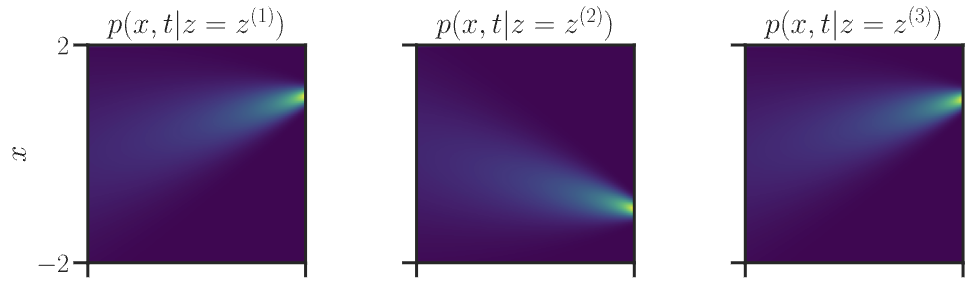
\includegraphics[width=\linewidth]{figs/conical_paths}
	\end{figure}
	\myfootnotewithlink{https://dl.heeere.com/conditional-flow-matching/blog/conditional-flow-matching}{image credit: A Visual Dive into Conditional Flow Matching}
\end{frame}
%=======
\begin{frame}{Summary}
	\begin{itemize}
		\item Conditional flow matching allows to make the FM objective tractable.
	\end{itemize}
\end{frame}
\end{document} 